\documentclass[a4paper]{article}
\usepackage[spanish]{babel}
\usepackage[utf8]{inputenc}
\usepackage{fancyhdr}
\usepackage{charter} % tipografia
%\usepackage{graphicx}
\usepackage{bytefield}
\usepackage[pdftex]{graphicx}
\usepackage{bm} % bold font in math mode
\usepackage{sidecap}
\usepackage{caption}
\usepackage{subcaption}
\usepackage{booktabs}
\usepackage{makeidx}
\usepackage{float}
\usepackage{amsmath, amsthm, amssymb}
\newtheorem{theorem}{Teorema}
\newtheorem{customthm}{Teorema}
\newtheorem{corollary}{Corolario}[theorem]
\newtheorem{proposition}[theorem]{Proposición}
\newtheorem{innercustomlemma}{Lemma}
\newenvironment{customlemma}[1]
  {\renewcommand\theinnercustomlemma{#1}\innercustomlemma}
  {\endinnercustomlemma}
\usepackage{amsfonts}
\usepackage{sectsty}
\usepackage{wrapfig}
\usepackage{listings}
\usepackage{hyperref} % links
\usepackage{algorithm} %http://www.ctan.org/pkg/algorithms
\usepackage{algorithmic}
\usepackage[usenames,dvipsnames]{xcolor}
\usepackage{pgfplotstable}
\usepackage{pgfplots}
\usepackage{tabularx} % tablas copadas
% custom
\usepackage{color} % para snipets de codigo coloreados
\usepackage{fancybox} % para el sbox de los snipets de codigo
\definecolor{litegrey}{gray}{0.94}
% \newenvironment{sidebar}{%
% \begin{Sbox}\begin{minipage}{.85\textwidth}}%
% {\end{minipage}\end{Sbox}%
% \begin{center}\setlength{\fboxsep}{6pt}%
% \shadowbox{\TheSbox}\end{center}}
% \newenvironment{warning}{%
% \begin{Sbox}\begin{minipage}{.85\textwidth}\sffamily\lite\small\RaggedRight}%
% {\end{minipage}\end{Sbox}%
% \begin{center}\setlength{\fboxsep}{6pt}%
% \colorbox{litegrey}{\TheSbox}\end{center}}

%\newenvironment{codesnippet}{%
%\begin{Sbox}\begin{minipage}{\linewidth-2\fboxsep-2\fboxrule-4pt}\sffamily\small}%
%{\end{minipage}\end{Sbox}%
%\begin{center}%
%\colorbox{litegrey}{\TheSbox}\end{center}}

% \newenvironment{codesnippet}{\VerbatimEnvironment%
%   \noindent
%   %{\columnwidth-\leftmargin-\rightmargin-2\fboxsep-2\fboxrule-4pt}
%   \begin{Sbox}
%   \begin{minipage}{\linewidth-2\fboxsep-2\fboxrule-4pt}
%   \begin{Verbatim}
% }{%
%   \end{Verbatim}
%   \end{minipage}
%   \end{Sbox}%
%   \colorbox{litegrey}{\TheSbox}
% }

\newenvironment{codesnippet}{%
  \noindent
  %      {\columnwidth-\leftmargin-\rightmargin-2\fboxsep-2\fboxrule-4pt}
  \begin{Sbox}
  \begin{minipage}{\linewidth}
  \begin{lstlisting}
}{
  \end{lstlisting}
  \end{minipage}
  \end{Sbox}%
  \colorbox{litegrey}{\TheSbox}
}

\usepackage{fancyhdr}
\pagestyle{fancy}
%\renewcommand{\chaptermark}[1]{\markboth{#1}{}}
\renewcommand{\sectionmark}[1]{\markright{\thesection\ - #1}}
\fancyhf{}
\fancyhead[LO]{Sección \rightmark} % \thesection\
\fancyfoot[LO]{\small{Iv\'an Arcuschin, Mart\'in Jedwabny, Jos\'e Massigoge, Iv\'an Pondal}}
\fancyfoot[RO]{\thepage}
\renewcommand{\headrulewidth}{0.5pt}
\renewcommand{\footrulewidth}{0.5pt}
\setlength{\hoffset}{-0.8in}
\setlength{\textwidth}{16cm}
%\setlength{\hoffset}{-1.1cm}
%\setlength{\textwidth}{16cm}
\setlength{\headsep}{0.5cm}
\setlength{\textheight}{25cm}
\setlength{\voffset}{-0.7in}
\setlength{\headwidth}{\textwidth}
\setlength{\headheight}{13.1pt}
\renewcommand{\baselinestretch}{1.1} % line spacing

% -------------------- COMANDOS ESPECIALES ------------------------------

\newcommand{\calcular}[2]{\pgfmathtruncatemacro{#1}{#2}}

\pgfplotsset{
  filter params/.style n args={4}{
      x filter/.code={
          \edef\tempa{\thisrow{#1}}
          \edef\tempb{#2}
          \edef\tempc{\thisrow{#3}}
          \edef\tempd{#4}
          \ifx\tempa\tempb
            \ifx\tempc\tempd
            \else
              \def\pgfmathresult{inf}
            \fi
          \else
            \def\pgfmathresult{inf}
          \fi
      }
  }
}

\newcommand{\graficarDatos}[6]{
  \begin{tikzpicture}
  \begin{axis}[
      title={#1},
      xlabel={#2},
      ylabel={#3},
      scaled x ticks=false,
      scaled y ticks=false,
      scale=0.5
  ]
  \addplot[only marks, color=black] table[x=#4,y=#5]{#6};
  \end{axis}
  \end{tikzpicture}
}

\newcommand{\graficarDatosPlus}[7]{
  \begin{tikzpicture}
  \begin{axis}[
      title={#1},
      xlabel={#2},
      ylabel={#3},
      scaled x ticks=false,
      scaled y ticks=false,
      width=0.6\textwidth,
      #7
  ]
  \addplot[only marks, color=black] table[x=#4,y=#5]{#6};
  \end{axis}
  \end{tikzpicture}
}

\makeatletter
\pgfplotsset{
    groupplot xlabel/.initial={},
    every groupplot x label/.style={
        at={($({group c1r\pgfplots@group@rows.west}|-{group c1r\pgfplots@group@rows.outer south})!0.5!({group c\pgfplots@group@columns r\pgfplots@group@rows.east}|-{group c\pgfplots@group@columns r\pgfplots@group@rows.outer south})$)},
        anchor=north,
    },
    groupplot ylabel/.initial={},
    every groupplot y label/.style={
            rotate=90,
        at={($({group c1r1.north}-|{group c1r1.outer
west})!0.5!({group c1r\pgfplots@group@rows.south}-|{group c1r\pgfplots@group@rows.outer west})$)},
        anchor=south
    },
    execute at end groupplot/.code={%
      \node [/pgfplots/every groupplot x label]
{\pgfkeysvalueof{/pgfplots/groupplot xlabel}};
      \node [/pgfplots/every groupplot y label]
{\pgfkeysvalueof{/pgfplots/groupplot ylabel}};
    },
    group/only outer labels/.style =
{
group/every plot/.code = {%
    \ifnum\pgfplots@group@current@row=\pgfplots@group@rows\else%
        \pgfkeys{xticklabels = {}, xlabel = {}}\fi%
    \ifnum\pgfplots@group@current@column=1\else%
        \pgfkeys{yticklabels = {}, ylabel = {}}\fi%
}
}
}

\def\endpgfplots@environment@groupplot{%
    \endpgfplots@environment@opt%
    \pgfkeys{/pgfplots/execute at end groupplot}%
    \endgroup%
}
\makeatother

\newcommand{\barGraphExp}[2]{
    \begin{tikzpicture}
    \begin{axis}[
        xlabel={Implementación},
    	ylabel={Tiempo de ejecución (clocks)},
        legend style={at={(1.4,1.0)}},
        ybar,
        scaled ticks=false,
        width=0.5\textwidth,
        height=0.5\textwidth,
        tickpos=left,
        xtick=\empty,
        ytick align=inside,
        xtick align=inside,
    	enlargelimits=0.05,
        bar width=16,
    ]
    % How to process each item:
    \renewcommand*{\do}[1]{\addplot+[color=black] table[x=n, y=##1]{datos/datos_blur.dat};}
    % Process list:
    \docsvlist{#2}
    \legend{#2}
    \end{axis}
    \end{tikzpicture}
}

\newcommand{\graficarDatosExp}[6]{
  \begin{tikzpicture}
  \begin{axis}[
      title={#1},
      xlabel={#2},
      ylabel={#3},
      scaled x ticks=false,
      scaled y ticks=false,
      enlargelimits=0.05,
      width=0.5\textwidth,
      height=0.5\textwidth
  ]
  \addplot[color=black] table[x=#5,y=#6]{#4};
  % \renewcommand*{\do}[1]{\addplot table[x=#5,y=##1]{#4};}
  % %     % Process list:
  % \docsvlist{#6}
  % \legend{#6}
  \end{axis}
  \end{tikzpicture}
}

% ------------------------------------------------------------------------

% \setcounter{secnumdepth}{2}
\usepackage{underscore}
\usepackage{kbordermatrix}% Matrix column labels
%\usetikzlibrary{arrows,shapes}
%\usepackage{tkz-graph}
\usepackage{caratula}
\usepackage{url}
\lstset{
    language=C++,
    basicstyle=\ttfamily,
    keywordstyle=\color{blue}\ttfamily,
    stringstyle=\color{red}\ttfamily,
    commentstyle=\color{ForestGreen}\ttfamily,
    morecomment=[l][\color{magenta}]{\#},
    literate={á}{{\'a}}1 {ó}{{\'o}}1 {é}{{\'e}}1 {í}{{\'i}}1 {ú}{{\'u}}1 {Á}{{\'A}}1 {Í}{{\'I}}1 {É}{{\'E}}1 {Ú}{{\'U}}1 {Ó}{{\'O}}1 {\ \ }{{\ }}1,
	breaklines=true,
	tabsize=2
}

\DeclareUnicodeCharacter{2212}{-}

% *********************** %
\usepackage{tikz}
\usetikzlibrary{graphs}
\usetikzlibrary{calc}
\usetikzlibrary{arrows}
\usetikzlibrary{matrix}
% Otros
\usepackage{arrayjobx}
\usepackage{enumitem}
\usepackage{multicol}
\usepackage{natbib}
\usepackage{etoolbox}
\usepackage{listingsutf8}
\lstset{inputencoding=utf8/latin1}
\usepackage{fancyvrb}
\usepackage{float}
\usepackage{abstract}
\newcommand{\subscript}[2]{$#1 _ #2$}


% ******************************************************** %
\begin{document}
\thispagestyle{empty}
\materia{Métodos Numéricos}
\submateria{Segundo Cuatrimestre de 2015}
\titulo{Trabajo Práctico III}
%\subtitulo{Grupo: }
\integrante{Iv\'an Arcuschin}{678/13}{iarcuschin@gmail.com}
\integrante{Mart\'in Jedwabny}{885/13}{martiniedva@gmail.com}
\integrante{Jos\'e Massigoge}{954/12}{jmmassigoge@gmail.com}
\integrante{Iv\'an Pondal}{078/14}{ivan.pondal@gmail.com}
\maketitle
\renewcommand{\abstractname}{Abstract}
\begin{abstract}
   Fact: baby's videos are funny. And they are even funnier when watched in \textit{slow motion}.

   In this work, we look at 4 different Interpolation methods to automatically generate
   \textit{slow motion} videos. This is achieved by interpolating some amount of new frames
   between each pair of original frames. Depending on the method, this procedure
   generates different levels of \textit{smoothness}.

   Once the methods are explained and implementation details are cleared out, we
   will present several experiments, namely in two categories. The first ones, will
   asure that the methods actually work, in the general case of function interpolation.
   The second ones, will provide different ways to compare the quality of the videos
   produced by each method.
\end{abstract}
\vspace{3em}
\renewcommand{\abstractname}{Resumen}
\begin{abstract}
   Hecho: los videos de bebes son graciosos. Y son mucho más gracios cuando se miran en
   \textit{slow motion}.

   En este trabajo, nos centraremos en 4 diferentes métodos de Interpolación para generar
   automaticamente videos en cámara lenta. Esto se logra interpolando una cierta
   cantidad de cuadros nuevos entre cada par de cuadros originales. Dependiendo del
   método, este procedimiento genera diferentes niveles de calidad.

   Una vez que hayamos explicado los métodos junto con su implementación, presentaremos
   varios experimentos, dentro de dos categorías. La primera, asegurará que los métodos
   funcionen correctamente, en el caso general de interpolación de funciones. La
   segunda, proveerá diferentes formas de comparar la calidad de los videos producidos
   por cada método.
\end{abstract}
\vspace{3em}
\textbf{Keywords:} Video, slow motion, interpolation methods, splines
% no footer on the first page
\thispagestyle{empty}
\newpage

\tableofcontents

\newpage
\section{Introducción}
 El objetivo principal de este Trabajo Práctico es estudiar, implementar y analizar
 métodos de Interpolación para generar Videos con \textit{slow motion}.

Comenzaremos haciendo una breve introducción a los distintos métodos de Interpolación,
para luego explicar cual es el modelo que subyace en cada uno:
\begin{itemize}
    \item Interpolación por Vecinos.
    \item Interpolación Fragmentaria Lineal.
    \item Interpolación por Splines.
    \item Interpolación por Splines (bloques de tamaño fijo).
\end{itemize}

Una vez finalizada la parte del Modelo, pasaremos a describir la Implementación de los
diferentes métodos presentados, realizadas en \texttt{C++}.

Ya llegando al final, pasaremos a presentar la Experimentación realizada, a la vez
que iremos analizando y discutiendo los resultados obtenidos.

Los experimentos realizados pueden dividirse en dos categorías. La primera, relacionada
con el costo temporal y la correctitud de los diversos algoritmos utilizados:
\begin{itemize}
    \item Funcionamiento de los métodos implementados al tratar de interpolar diferentes
        familias de funciones.
    \item Comparación de tiempos de ejecución entre los distintos métodos.
    \item Determinación del tamaño de bloque del método Interpolación por Splines.
\end{itemize}

La segunda, relacionada con el aspecto cualitativo de los métodos:
\begin{itemize}
    \item Comparación del \textit{Error Cuadrático Medio} y \textit{Peak to Signal Noise Rate} entre
        los distintos métodos.
    \item Análisis del fenómeno de Artifacts.
\end{itemize}

Para finalizar, cerraremos el presente informe con una conclusión, en la cual
discutiremos acerca de los métodos vistos, así como de la experimentación realizada.
También, contaremos las dificultades encontradas al realizar el Trabajo Práctico,
las posibles continuaciones que se podrían realizar, y si los objetivos planteados
fueron alcanzados.


\newpage
\section{Modelo}
\subsection{Video}

Definiremos un modelo para los videos con el cual sea fácil de trabajar a la hora de realizar
el \textit{slow motion}.
Dado un video, definiremos:
\begin{itemize}
    \item $w$ el ancho en píxeles de cada frame.
    \item $h$ el ancho en píxeles de cada frame.
    \item $f_i$ el $i$-ésimo frame, con $0< i < k$, donde k es la cantidad de frames totales.
    \item $p(x,y,f_i)$, con $0 < x < w$, $0< y < h$, el píxel en la posición $(x,y)$ del frame $f_i$.
\end{itemize}

Luego, si tomamos $p(x,y,f_i)$ y $p(x,y,f_{i+1})$ querremos agregar una cierta cantidad
de píxeles entre ambos, de forma que haya una transición del primero al segundo y
se produzca el \textit{slow motion}.

Para elegir que valores agregar entre los píxeles, utilizaremos diferentes métodos
de interpolación.
\begin{itemize}
    \item \textit{Vecinos}: Consiste en rellenar los nuevos frames replicando los
        valores de los píxeles del frame original que se encuentra más cerca.
    \item \textit{Interpolación Lineal}: Consiste en rellenar los píxeles utilizando
        interpolaciones lineales entre píxeles de frames originales consecutivos.
    \item \textit{Interpolación por Splines}: Consiste en rellenar los píxeles utilizando
        Splines entre píxeles de frames originales consecutivos. En este método,
        utilizaremos la información provista por todos los frames del video,
        y generaremos $k-1$ funciones, cada una de a lo sumo grado cúbico.
    \item \textit{Interpolación por Splines con tamaño de bloque variante}:
        Simliar al anterior, pero con la posibilidad de variar la cantidad de frames
        tomados en cuenta al generar las funciones.
\end{itemize}

En las siguientes secciones explicaremos con mayor detalle cada uno de los métodos.

\subsection{Vecinos}\label{Vecinos}
En este método, eligiremos para cada nuevo píxel el valor del frame original que se encuentre
más cercano.
Si definimos $c$ como la cantidad de frames a agregar entre cada par original, y
$g_0, \dots, g_{c-1}$ los nuevos frames. Tenemos que:
\begin{equation*}
    \begin{aligned}
        p(x,y,f_{i}) &= p(x,y,f_{i})\\
        p(x,y,g_{0}) &= p(x,y,f_{i})\\
        \vdots\\
        p(x,y,g_{c/2-1}) &= p(x,y,f_{i})\\
        p(x,y,g_{c/2}) &= p(x,y,f_{i+1})\\
        \vdots\\
        p(x,y,g_{c-1}) &= p(x,y,f_{i+1})\\
        p(x,y,f_{i+1}) &= p(x,y,f_{i+1})
    \end{aligned}
\end{equation*}

\subsection{Interpolación Lineal}\label{Lineal}
En este método, buscaremos interpolar los píxeles de frames contiguos con una función
lineal. Para ello, construiremos un Polinomio Interpolante de grado 1 utilizando
\textit{diferencias divididas}, ya que ofrece una construcción más sencilla que al seguir
el método de Lagrange.

Luego, si llamamos $f$ a la función (desconocida excepto en los puntos $x_j$), definimos:
\begin{itemize}
    \item Diferencia dividida de orden cero en $x_j$:
        \begin{equation*}
            f[x_j] = f(x_j)
        \end{equation*}
    \item Diferencia dividida de orden uno en $x_j$, $x_{j+1}$:
        \begin{equation*}
            f[x_j,x_{j+1}]= \frac{f[x_{j+1}] - f[x_j]}{x_{j+1} - x_j} = \frac{f(x_{j+1}) - f(x_j)}{x_{j+1} - x_j}
        \end{equation*}
    \item Polinomio Interpolante de grado 1 para $x_j$, $x_{j+1}$:
        \begin{equation*}
            P_1(x) = f[x_j] + f[x_j,x_{j+1}](x-x_j) = f(x_j) + \frac{f(x_{j+1}) - f(x_j)}{x_{j+1} - x_j}*(x-x_j)
        \end{equation*}
\end{itemize}

\subsection{Interpolación por Splines}\label{Splines}

\subsection{Interpolación por Splines con tamaño de bloque variante}\label{MultiSplines}


\newpage
\section{Implementación}\label{Implementacion}
\subsection{Interpolación por vecinos}

Este método consiste en reemplazar los cuadros intermedios a ser rellenados por el cuadro original mas cercano en el tiempo.
Es decir, dados los cuadros del video sin camara lenta, generamos otro video en camara lenta copiando los cuadros originales de la siguiente manera:

% \begin{bytefield}{16}
% \wordbox{1}{A 16-bit field} \\
% \bitbox{8}{8 bits} & \bitbox{8}{8 more bits} \\
% \wordbox{2}{A 32-bit field. Note that text wraps within the box.}
% \end{bytefield}

Sean Frame1 y Frame2 dos cuadros consecutivos del video original:

\begin{bytefield}{8}
\bitbox{4}{Frame1} & \bitbox{4}{Frame2}
\end{bytefield}

Si queremos ahora 6 cuadros entre cada 2 del archivo original lo transformamos a:

\begin{bytefield}{32}
\bitbox{4}{Frame1} & \bitbox{4}{Frame1} & \bitbox{4}{Frame1} & \bitbox{4}{Frame1} & \bitbox{4}{Frame2} & \bitbox{4}{Frame2} & \bitbox{4}{Frame2} & \bitbox{4}{Frame2}
\end{bytefield}

El pseudocódigo sería el siguiente:

\begin{lstlisting}
Sean W,H,I el ancho, alto y la cantidad de frames del video original
Sea video[W][H][I] el triple vector de numeros enteros que representa el video original
Sea K la cantidad de frames que queremos agregar entre cuadro y cuadro

Crear un triple vector de enteros new_video[W][H][I+(I-1)*K]
Para w = 0 hasta W-1 hacer
	Para h = 0 hasta H-1 hacer
		Para i = 0 hasta I-2 hacer
			Para j = 0 hasta K/2 hacer
				new_video[w][h].push_back(video[w][h][i])
			Fin para
			Para j = (K/2)+1 hasta K hacer
				new_video[w][h].push_back(video[w][h][i+1])
			Fin para
		Fin para
		new_video[w][h].push_back(video[w][h][I-1])
	Fin para
Fin para
Devolver new_video
\end{lstlisting}

\subsection{Interpolación lineal}

En este caso, usamos el polinomio interpolador de Lagrange entre cada par de puntos/pixeles consecutivos para aproximar los valores intermedios que irían en el video de camara lenta. Esto genera una función lineal para los pixeles consecutivos en la misma posición.

Por ejemplo, sean dos pixeles con valores 1 y 4:

\begin{bytefield}{8}
\bitbox{4}{1} & \bitbox{4}{4}
\end{bytefield}

Si queremos un video en camara lenta con 5 cuadros intermedios por cada 2 del original, estos se replicarán de la siguiente forma:

\begin{bytefield}{28}
\bitbox{4}{1} & \bitbox{4}{1.5} & \bitbox{4}{2} & \bitbox{4}{2.5} & \bitbox{4}{3} & \bitbox{4}{3.5} & \bitbox{4}{4}
\end{bytefield}

El procedimiento es el siguiente:

\begin{lstlisting}
Sean W,H,I el ancho, alto y la cantidad de frames del video original
Sea video[W][H][I] el triple vector de numeros enteros que representa el video original
Sea K la cantidad de frames que queremos agregar entre cuadro y cuadro

Crear un triple vector de enteros new_video[W][H][I+(I-1)*K]
Para w = 0 hasta W-1 hacer
	Para h = 0 hasta H-1 hacer
		Para i = 0 hasta I-2 hacer
			coef_cero = video[w][h][i]
			coef_uno = (video[w][h][i+1] - video[w][h][i]) / (K+1);
			Para k = 0 hasta K hacer
				pixel = coef_cero + coef_uno*k;
				Si (pixel < 0) pixel = 0
				Si (pixel > 255) pixel = 255
				new_video.push_back(pixel)
		Fin para
		new_video.push_back(video[w][h][I-1])
	Fin para
Fin para
Devolver new_video
\end{lstlisting}

\subsection{Interpolación por Splines}

En este método aplicamos la técnica de Splines. Esta consiste en generar un sistema de ecuaciones para encontrar una función por partes que interpole cada par de puntos con polinomios de forma que la curva resultante sea continua y dos veces derivable. Como el sistema es tridiagonal, podemos aprovechar para guardar los valores de la matriz de forma más eficiente. El pseudocódigo es el siguiente:

\begin{lstlisting}
Sean W,H,I el ancho, alto y la cantidad de frames del video original
Sea video[W][H][I] el triple vector de numeros enteros que representa el video original
Sea K la cantidad de frames que queremos agregar entre cuadro y cuadro

Crear un triple vector de enteros new_video[W][H][I+(I-1)*K]
Para w = 0 hasta W-1 hacer
	Para h = 0 hasta H-1 hacer
		new_video[w][h] = GenerarSpline(video[w][h])
	Fin para
Fin para
Devolver new_video

GenerarSpline(y[n]):
	Crear un vector de enteros valores[I+(I-1)*K]
	Crear doble vector de enteros sistema[n][2]
	sistema[0] = {1,0}
	Para j = 1 hasta n-2 hacer
		sistema[j] = {1, 4}
	Fin para
	sistema[n-1] = {0,1}
	// Factorización LU
	Para j = 1 hasta n-2 hacer
		coef = sistema[i + 1][0]/sistema[i][1];
		sistema[i + 1][0] = coef
		sistema[i + 1][1] -= coef
	Fin para
	Crear vectores x[n], a[n], b[n], c[n], d[n]
	a = y
	Para i = 1 hasta n-2 hacer
		x[i] = 3*(a[i + 1] - 2*a[i] + a[i - 1]);
		x[i] -= x[i - 1]*sistema[i][0];
	Fin para
	// Resuelvo triangular superior (Uc = x)
	Para i = n - 2 hasta 1 hacer
		c[i] = x[i];
		c[i] -= c[i + 1];
		c[i] /= sistema[i][1];
	Fin para
	// Calculo mis coeficientes "b" y "d"
	Para i = 0 hasta n-2 hacer
		b[i] = a[i + 1] - a[i] - (2*c[i] + c[i + 1])/3;
		d[i] = (c[i + 1] - c[i])/3;
	Fin para
	//Calculo los pixeles resultantes con el Spline
	Para i = 0 hasta n-1 hacer
		Para j = 0 hasta K hacer
			dif = j/(K+1)
			val = a[i] + b[i]*(dif) + c[i]*(dif)*(dif) + d[i]*(dif)*(dif)*(dif)
			valores.push_back(val)
		Fin para
	Fin para
	valores.push_back(y[n-1])
	Devolver valores
\end{lstlisting}

\subsection{Interpolación por Splines de a bloques}

A diferencia del método anterior, en este caso vamos a querer aplicar la técnica de Splines a bloques de pixeles de tamaño fijo. Es decir, para una misma posición del video, en vez de utilizar todos los valores del pixel a través del tiempo, generamos splines entre particiones de la misma longitud. El procedimiento es:

\begin{lstlisting}
Sean W,H,I el ancho, alto y la cantidad de frames del video original
Sea video[W][H][I] el triple vector de numeros enteros que representa el video original
Sea K la cantidad de frames que queremos agregar entre cuadro y cuadro
Sea T el tamano de bloque de los Splines
Observacion: reutilizamos el metodo GenerarSpline(y) de los Splines normales
Observacion: asumimos que I es divisible por T para simplificar este pseudocodigo

Crear un triple vector de enteros new_video[W][H][I+(I-1)*K]
Para w = 0 hasta W-1 hacer
	Para h = 0 hasta H-1 hacer
		Para t = 0 hasta T-1 hacer
			Crear subarreglo aux[T] = video[w][h][T*t..T*(t+1)-1]
			Crear arreglo bloque[T] = GenerarSpline(aux)
			Pushear a new_video[w][h] todos los valores de 'bloque'
		Fin para
	Fin para
Fin para
Devolver new_video
\end{lstlisting}

\newpage
\section{Experimentación}
En esta sección, se detallan los diferentes experimentos que realizamos para medir el funcionamiento, la eficiencia y calidad de resultados, tanto de forma cuantitativa como cualitativa, de los métodos implementados.

Para lograr tal fin realizamos los siguientes tipos de experimentos:
\begin{itemize}
  \item Funcionamiento de los métodos implementados: Mostraremos que los métodos
        de interpolación funcionan correctamente comparandolos contra diferentes
        familias de funciones. A su vez, basandonos en las precisiones obtenidas,
        determinaremos el tamaño de bloque óptimo para el método Interpolación por Splines.
  \item Medición del ECM y PSNR de los métodos: Compararemos los errores obtenidos
        en varias instancias de pruebas para los distintos métodos.
  \item Medición de los tiempos de ejecución de los métodos: Compararemos los
        tiempos de ejecución utilizando los distintos métodos.
  \item Análisis cualitativos de los métodos, fenómeno de artifacts: Buscaremos
        reconocer defectos de interpolación en los videos generados.
\end{itemize}

Los videos utilizados para los diversos experimentos, fueron los siguientes:

\begin{itemize}
  \item \textbf{Video 1 - Skate}: 426x240, cantidad de cuadros originales: 151 , fps: 30, duracion: 5s.
  \item \textbf{Video 2 - Messi}: 426x240, cantidad de cuadros originales: 151, fps: 30, duracion: 5s.
  \item \textbf{Video 3 - Amanecer}: 426x240, cantidad de cuadros originales: 151, fps: 30, duracion: 5s.
\end{itemize}

Es importante mencionar que cada video representa una clase de video distinto, en donde el Video 1 contiene movimientos bruscos, el Video 2 cambios de camara, y el Video 3 movimientos suaves.

El motivo de estas elecciones se debe a la busqueda de diversos \textit{artifacts} a partir de las caracteristicas de cada clase.

\subsection{Detalles generales de la experimentación}

\begin{itemize}
    \item En los experimentos que se utilizaron números aleatorios, se generaron utilizando la función \textit{rand}, provista por la librería \texttt{stdlib.h}.
    \item La semilla para los números aleatorios se seteo utilizando el método \textit{srand(time(NULL))}, para evitar repeticiones de números en diferentes corridas.
    \item Las instancias de prueba fueron generadas con los archivos provistos por la cátedra. Adicionalmente, hicimos nuestras propias instancias emulando diferentes funciones (por ejemplo una función constante, lineal y cuadrática) para realizar el control de calidad de los métodos.
    \item Para medir los tiempos utilizamos la librería \textit{chrono} y medimos los resultados en nanosegundos.
    \item A su vez, utilizamos el nivel de optimización \textit{O2} de \textit{C++} a la hora de compilar el código.
    \item Todos los tests fueron corridos en la misma máquina bajo las mismas condiciones.
\end{itemize}


\subsection{Funcionamiento de los métodos implementados}\label{exp_funcionamiento}
En este experimento nuestro objetivo fue asegurarnos el correcto funcionamiento de nuestra implementación de la interpolación fragmentaria lineal, interpolación por splines, e interpolación por splines con tamaño de bloque fijo, tomando bloques de 2, 4, 8, 16, 32 y 64 cuadros.

Con este fin, realizamos una serie de tests que muestran el correcto funcionamiento de cada método para distintas familias de funciones:
\begin{itemize}
  \item Función constante.
  \item Función lineal.
  \item Función cuadrática.
  \item Función cúbica.
\end{itemize}

Luego, cada método de interpolación fue testeado contra cada una de las familias de funciones mencionadas de la siguiente forma:
\begin{itemize}
  \item Dada una familia de funciones, se generan aleatoriamente los coeficientes necesarios para definir una función de esa familia, i.e.: para una constante se genera solo el coeficiente independiente, mientras que para una cuadrática se generan 3 coeficientes.
    \item Una vez generada la función, se la evalua en un rango de valores para obtener un array de valores esperados.
    \item Luego, a partir del array de valores esperados se construye otro array quitandole elementos a intervalos fijos.
        Este nuevo array será el utilizado para realizar la interpolación, y lo que testearemos es la aproximación de  la
        interpolación a los elementos que quitamos.
    \item Una vez que tenemos la interpolación con cualquiera de los métodos mencionados, basta recorrer los elementos del array de valores esperados a la vez que evaluamos la interpolación obtenida.
        Para cada par de valores: esperado e interpolado, querremos ver que la diferencia absoluta es menor que un epsilon/cota de precision que
        definiremos dependiendo del método utilizado y la función a interpolar.
\end{itemize}

Es importante mencionar algunas carácterísticas de las instancias utilizadas:
\begin{itemize}
    \item Cantidad de puntos generados con la función(tamaño del array de valores esperados): 100
    \item Cantidad de puntos a interpolar: 50.
    \item Todos los coeficientes generados aleatoriamente están en el rango $[1,10]$,
        para evitar que las funciones generadas crezcan de forma desmedida.
\end{itemize}

Luego, se obtuvieron las siguientes cotas de precisión para los distintos métodos y funciones:

\begin{table}[H]
    \begin{tabular}{| c | c | c | c | c |}
    \hline
    {} & F. Constante & F. Lineal & F. Cuadrática & F. Cúbica \\ \hline
    Interpolación por Vecinos & 0.0001 & 10 & 1000 & 100000 \\
    Interpolación Fragmentaria Lineal & 0.0001 & 0.0001 & 10 & 1000 \\
    Interpolación por Splines (bloques tamaño 2) & 0.0001 & 0.0001 & 10 & 1000 \\
    Interpolación por Splines (bloques tamaño 4) & 0.0001 & 0.0001 & 5 & 500 \\
    Interpolación por Splines (bloques tamaño 8) & 0.0001 & 0.0001 & 1 & 200 \\
    Interpolación por Splines (bloques tamaño 16) & 0.0001 & 0.0001 & 1 & 200 \\
    Interpolación por Splines (bloques tamaño 32) & 0.0001 & 0.0001 & 1 & 200 \\
    Interpolación por Splines (bloques tamaño 64) & 0.0001 & 0.0001 & 1 & 200 \\
    Interpolación por Splines (1 solo bloque) & 0.0001 & 0.0001 & 1 & 200 \\
    \hline
    \end{tabular}
\end{table}

Analizando dichas cotas vemos que:
\begin{itemize}
    \item La Interpolación por Vecinos resulta razonable solo para funciones con muy
        poca variación (derivada a lo sumo constante). Esto se ve claramente en la
        cota de presición al interpolar una función Cuadrática.
    \item La Interpolación Fragmentaria Lineal es sustancialmente mejor que por Vecinos,
        y devuelve resultados razonables para funciones a lo sumo Cuadráticas.
    \item La Interpolación por Splines utilizando solo 2 puntos para cada bloque es
        equivalente a interpolar utilizando funciones lineales, y queda evidenciado al
        tener las mismas cotas de precisión.
    \item A partir de los tamaños de bloque 4 a 16, la Interpolación por Splines realiza
        una mejora ``asintótica'' de su cota de precisión.
    \item Entre los tamaños de bloque 16 a 64, no se notó una mejora significativa en la cota
        de precisión de la Interpolación por Splines.
    \item Al realizar Interpolación por Splines \textit{standard} (1 solo bloque),
        vemos que su cota de precisión concuerda con las cotas a las cuales ``convergen''
        los métodos de Interpolación por Splines con bloque de tamaño fijo. Es por esta razón
        que para los experimentos cualitativos, utilizaremos solamente la Interpolación
        por Splines \textit{standard}, y no la de tamaño de bloques fijo.
\end{itemize}

\subsection{Medición de los tiempos de ejecución de los métodos}
A partir de la implementaciones descriptas en la Sección \ref{Implementacion},
podemos inferir una complejidad temporal para cada método.

Sea $w$ la cantidad de filas de píxeles en cada imagen, $h$ la cantidad de
columnas, $i$ la cantidad de cuadros originales y sea $k$ la cantidad de
cuadros a agregar entre los originales:

Todos los metodos implementados tienen la misma complejidad temporal que es
 $\Theta(w*h*i*k*)$. Esta conclusion surge del hecho de que, en todos los casos,
 tenemos 4 ciclos anidados, en donde el primero se ejecuta $w$ veces, el segundo
 $h$ veces, el tercero $i$ veces, y el cuarto $k$ veces.
%\begin{itemize}
%  \item Vecino mas cercano: realizamos 4 ciclos anidados, en donde el primero se ejecuta $w$ veces, el segundo $h$ veces, el tercero $i$ veces, y el cuarto $k$ veces, la complejidad temporal del mismo es $\Theta(whik)$.
%  \item Interpolacion lineal: situacion identica a la de vecinos mas cercanos, por lo tanto su complejidad temporal es de $\Theta(whik)$.
%  \item Interpolacion por Splines: en este caso realizamos primero un ciclo que se ejecuta $w$ veces, dentro de este ciclamos $h$
%  \item Interpolacion por Splines con tamaño de bloque fijo:
%\end{itemize}
\newline
\newline
Para corroborar esta hipotesis planteamos un experimento con las siguientes caracteristicas:
\begin{itemize}
  \item Utilizamos el video provisto por la catedra llamado \textit{funnybaby}, el cual tiene 44 cuadros y es de 240x320.
  \item Solo medimos la resolucion del sistema, no su creacion o los respectivos pasajes de video a texto y viceversa.
  \item Dado que $w$, $h$ y $i$ son valores fijos que no podemos cambiar, variamos el $k$.
  \item Generamos instancias para valores de $k$ entre 1 y 6.
  \item Para cada valor distinto de $k$ generamos 4 instancias, cuyos valores vamos a promediar para mitigar los posibles valores distorsionados por algun procedimiento del procesador.
\end{itemize}

Los resultamos obtenidos fueron los siguientes:

\begin{center}
    \begin{tikzpicture}
    \begin{axis}[
        title={},
        xlabel={cantidad de cuadros agregados entre originales ($k$)},
        ylabel={tiempo (nanosegundos)},
        ylabel absolute,
        ylabel style={yshift=.3cm},
        scaled x ticks=false,
        scaled y ticks=false,
        enlargelimits=0.05,
        width=0.85\textwidth,
        height=0.45\textwidth,
        legend style={at={(1.015,1)},anchor=north west},
        no markers,
        thick,
        cycle list name=exotic
    ]
    \addplot[color=green] table[x index=0,y index=1]{datos/timelineal};
    \addplot[color=red] table[x index=0,y index=1]{datos/timevecinos};
    \addplot[color=blue] table[x index=0,y index=1]{datos/timesplines};
    \legend{Lineal, Vecinos, Splines}
    \end{axis}
    \end{tikzpicture}
\end{center}

Si tomamos los tiempos que arrojó la experimentación, y los dividimos por su respectivo $k$, obtenemos el siguiente resultado:

\begin{center}
    \begin{tikzpicture}
    \begin{axis}[
        title={},
        xlabel={cantidad de cuadros agregados entre originales ($k$)},
        ylabel={tiempo (nanosegundos) / $k$},
        ylabel absolute,
        ylabel style={yshift=.3cm},
        scaled x ticks=false,
        scaled y ticks=false,
        enlargelimits=0.05,
        width=0.85\textwidth,
        height=0.45\textwidth,
        legend style={at={(1.015,1)},anchor=north west},
        no markers,
        thick,
        cycle list name=exotic
    ]
    \addplot[color=green] table[x index=0,y index=2]{datos/timelineal};
    \addplot[color=red] table[x index=0,y index=2]{datos/timevecinos};
    \addplot[color=blue] table[x index=0,y index=2]{datos/timesplines};
    \legend{Lineal, Vecinos, Splines}
    \end{axis}
    \end{tikzpicture}
\end{center}

A partir de los graficos, queda de manifiesto que los metodos tienen la misma complejidad temporal, ya que solo difieren en una constante.

\subsection{Medición del ECM y PSNR de los métodos.}\label{ECM}
Sea $F$ un frame del vídeo real (ideal) , y $\bar{F}$ el mismo frame del vídeo efectivamente construidos por alguno de los métodos. Sea $m$ la cantidad de filas de píxeles en cada imagen y $n$ la cantidad de columnas.

Definimos el Error Cuadrático Medio, \texttt{ECM}, como el real dado por:
\begin{equation}
\texttt{ECM}(F,\bar{F}) = \frac{1}{mn}\sum_{i=1}^m\sum_{j = 1}^n |F_{k_{ij}} - \bar{F}_{k_{ij}}|^2
\end{equation}

A su vez definimos \emph{Peak to Signal Noise Ratio}, \texttt{PSNR}, como el real dado por:
\begin{equation}
\texttt{PSNR}(F,\bar{F}) = 10 \log_{10}\bigg(\frac{255^2}{\texttt{ECM}(F,\bar{F})}\bigg). \label{eq:psnr}
\end{equation}

Ambas medidas nos sirven para realizar un análisis cuantitativo de la calidad de los resultados obtenidos con los distintos métodos.

En este experimento utilizamos los videos propuestos al inicio de la experimentacion, variando la cantidad de cuadros que agregamos.
Dichos videos fueron elegidos especificamente para variar la dificultad de Interpolación:
\begin{itemize}
    \item El video \textbf{Amanecer} no contiene movimientos bruscos ni cambios de cámaras
        por lo que, para cualquier método, el error debería ser en lineas generales
        menor que pare el resto de los videos.
    \item El video \textbf{Skate} contiene movimientos bruscos pero no cambios de cámaras
        por lo que, se espera un mayor error que en el video anterior. Además,
        deberíamos ver un aumento del error en los frames donde hay movimientos
        bruscos.
    \item El video \textbf{Skate} contiene movimientos bruscos y cambios de cámaras
        por lo que, se espera un mayor error que en el resto de los videos. Además,
        deberíamos ver un aumento \textit{importante} del error en los frames
        donde se produce el cambio de cámara.
\end{itemize}

A continuación, presentaremos e iremos analizando los resultados obtenidos:

\subsubsection{ECM - Agregando 1 cuadro}

\begin{figure}[H]
	\centering
	\begin{tikzpicture}
		\begin{axis}[
			title={ },
			xlabel=Frame,
			ylabel=ECM,
			width=0.8\textwidth,
			height=0.5\textwidth,
			yticklabel style={/pgf/number format/fixed},
			scaled y ticks=false,
			legend style={at={(1.015,1)},anchor=north west},
			no markers,
			thick,
            cycle list name=exotic
		]
		\addplot table[x index=0,y index=1]{../src/exp/error-sunrise-vecinos1};
        \addplot[color=blue] table[x index=0,y index=1]{../src/exp/error-sunrise-lineal1};
        \addplot[color=red] table[x index=0,y index=1]{../src/exp/error-sunrise-spline1};
		\legend{Vecinos, Lineal, Spline}
		\end{axis}
	\end{tikzpicture}
	\caption{ECM para el video \textbf{Amanecer} al agregar 1 cuadro con distintos métodos de Interpolación.}
	\label{fig:ecm_sunrise_1}
\end{figure}

\begin{figure}[H]
	\centering
	\begin{tikzpicture}
		\begin{axis}[
			title={ },
			xlabel=Frame,
			ylabel=ECM,
			width=0.8\textwidth,
			height=0.5\textwidth,
			yticklabel style={/pgf/number format/fixed},
			scaled y ticks=false,
			legend style={at={(1.015,1)},anchor=north west},
			no markers,
			thick,
			cycle list name=exotic
		]
		\addplot table[x index=0,y index=1]{../src/exp/error-skate-vecinos1};
        \addplot[color=blue] table[x index=0,y index=1]{../src/exp/error-skate-lineal1};
        \addplot[color=red] table[x index=0,y index=1]{../src/exp/error-skate-spline1};
		\legend{Vecinos, Lineal, Spline}
		\end{axis}
	\end{tikzpicture}
	\caption{ECM para el video \textbf{Skate}  al agregar 1 cuadro con distintos métodos de Interpolación.}
	\label{fig:ecm_skate_1}
\end{figure}

\begin{figure}[H]
	\centering
	\begin{tikzpicture}
		\begin{axis}[
			title={ },
			xlabel=Frame,
			ylabel=ECM,
			width=0.8\textwidth,
			height=0.5\textwidth,
			yticklabel style={/pgf/number format/fixed},
			scaled y ticks=false,
			legend style={at={(1.015,1)},anchor=north west},
			no markers,
			thick,
			cycle list name=exotic
		]
		\addplot table[x index=0,y index=1]{../src/exp/error-messi-vecinos1};
        \addplot[color=blue] table[x index=0,y index=1]{../src/exp/error-messi-lineal1};
        \addplot[color=red] table[x index=0,y index=1]{../src/exp/error-messi-spline1};
		\legend{Vecinos, Lineal, Spline}
		\end{axis}
	\end{tikzpicture}
	\caption{ECM para el video \textbf{Messi}  al agregar 1 cuadro con distintos métodos de Interpolación.}
	\label{fig:ecm_messi_1}
\end{figure}

Viendo las Figuras \ref{fig:ecm_sunrise_1}, \ref{fig:ecm_skate_1} y \ref{fig:ecm_messi_1} podemos decir que:
\begin{itemize}
    \item La Interpolación por Vecinos obtiene consistentemente un mayor error que
        el resto de los métodos.
    \item La Interpolación Fragmentaria Lineal y la Interpolación por Splines obtienen
        en general un error similar, siendo la primera ligeramente mejor.
    \item El rango de error obtenido por todos los métodos en el video \textbf{Amanecer},
        es significativamente menor que en el resto de los videos. Además, se puede ver
        que el error obtenido en ese video es en cierta forma ``regular'', lo cual
        tiene sentido ya que tiene movimientos suaves y repetitivos.
    \item El rango de error obtenido por todos los métodos en los videos \textbf{Skate} y \textbf{Messi},
        son similares, y ambos mayores al rango obtenido en el video \textbf{Amanecer}.
    \item El error obtenido en el video \textbf{Skate} es bastante irregular
        al compararlo con el video \textbf{Amanecer}, encontrandose un pico de error
        en el movimiento más brusco del video.
    \item A diferencia del caso anterior, el error obtenido en el video \textbf{Messi}
        es bastante regular, a excepción del pico de error que encontramos cuando
        ocurre el cambio de cámara, el cual es notorio para todos los métodos.
\end{itemize}

\subsubsection{PSNR - Agregando 1 cuadro}
\begin{figure}[H]
	\centering
	\begin{tikzpicture}
		\begin{axis}[
			title={ },
			xlabel=Frame,
			ylabel=PSNR,
			width=0.8\textwidth,
			height=0.5\textwidth,
			yticklabel style={/pgf/number format/fixed},
			scaled y ticks=false,
			legend style={at={(1.015,1)},anchor=north west},
			no markers,
			thick,
			cycle list name=exotic
		]
		\addplot table[x index=0,y index=2]{../src/exp/error-sunrise-vecinos1};
        \addplot[color=blue] table[x index=0,y index=2]{../src/exp/error-sunrise-lineal1};
        \addplot[color=red] table[x index=0,y index=2]{../src/exp/error-sunrise-spline1};
		\legend{Vecinos, Lineal, Spline}
		\end{axis}
	\end{tikzpicture}
	\caption{PSNR para el video \textbf{Amanecer} al agregar 1 cuadro con distintos métodos de Interpolación.}
	\label{fig:psnr_sunrise_1}
\end{figure}

\begin{figure}[H]
	\centering
	\begin{tikzpicture}
		\begin{axis}[
			title={ },
			xlabel=Frame,
			ylabel=PSNR,
			width=0.8\textwidth,
			height=0.5\textwidth,
			yticklabel style={/pgf/number format/fixed},
			scaled y ticks=false,
			legend style={at={(1.015,1)},anchor=north west},
			no markers,
			thick,
			cycle list name=exotic
		]
		\addplot table[x index=0,y index=2]{../src/exp/error-skate-vecinos1};
        \addplot[color=blue] table[x index=0,y index=2]{../src/exp/error-skate-lineal1};
        \addplot[color=red] table[x index=0,y index=2]{../src/exp/error-skate-spline1};
		\legend{Vecinos, Lineal, Spline}
		\end{axis}
	\end{tikzpicture}
	\caption{PSNR para el video \textbf{Skate} al agregar 1 cuadro con distintos métodos de Interpolación.}
	\label{fig:psnr_skate_1}
\end{figure}

\begin{figure}[H]
	\centering
	\begin{tikzpicture}
		\begin{axis}[
			title={ },
			xlabel=Frame,
			ylabel=PSNR,
			width=0.8\textwidth,
			height=0.5\textwidth,
			yticklabel style={/pgf/number format/fixed},
			scaled y ticks=false,
			legend style={at={(1.015,1)},anchor=north west},
			no markers,
			thick,
			cycle list name=exotic
		]
		\addplot table[x index=0,y index=2]{../src/exp/error-messi-vecinos1};
        \addplot[color=blue] table[x index=0,y index=2]{../src/exp/error-messi-lineal1};
        \addplot[color=red] table[x index=0,y index=2]{../src/exp/error-messi-spline1};
		\legend{Vecinos, Lineal, Spline}
		\end{axis}
	\end{tikzpicture}
	\caption{PSNR para el video \textbf{Messi} al agregar 1 cuadro con distintos métodos de Interpolación.}
	\label{fig:psnr_messi_1}
\end{figure}

Sabiendo que, mientras más grande es el \texttt{ECM} más chico es el \texttt{PSNR},
encontramos que la información provista por este último no aporta nuevos elementos
al análisis, ya que se condice con lo análizado previamente utilizando el \texttt{ECM}.

\subsubsection{ECM - Agregando 5 cuadros}

\begin{figure}[H]
	\centering
	\begin{tikzpicture}
		\begin{axis}[
			title={ },
			xlabel=Frame,
			ylabel=ECM,
			width=0.8\textwidth,
			height=0.5\textwidth,
			yticklabel style={/pgf/number format/fixed},
			scaled y ticks=false,
			legend style={at={(1.015,1)},anchor=north west},
			no markers,
			thick,
			cycle list name=exotic
		]
		\addplot table[x index=0,y index=1]{../src/exp/error-sunrise-vecinos5};
        \addplot[color=blue] table[x index=0,y index=1]{../src/exp/error-sunrise-lineal5};
        \addplot[color=red] table[x index=0,y index=1]{../src/exp/error-sunrise-spline5};
		\legend{Vecinos, Lineal, Spline}
		\end{axis}
	\end{tikzpicture}
	\caption{ECM para el video \textbf{Amanecer} al agregar 5 cuadros con distintos métodos de Interpolación.}
	\label{fig:ecm_sunrise_5}
\end{figure}

\begin{figure}[H]
	\centering
	\begin{tikzpicture}
		\begin{axis}[
			title={ },
			xlabel=Frame,
			ylabel=ECM,
			width=0.8\textwidth,
			height=0.5\textwidth,
			yticklabel style={/pgf/number format/fixed},
			scaled y ticks=false,
			legend style={at={(1.015,1)},anchor=north west},
			no markers,
			thick,
			cycle list name=exotic
		]
		\addplot table[x index=0,y index=1]{../src/exp/error-skate-vecinos5};
        \addplot[color=blue] table[x index=0,y index=1]{../src/exp/error-skate-lineal5};
        \addplot[color=red] table[x index=0,y index=1]{../src/exp/error-skate-spline5};
		\legend{Vecinos, Lineal, Spline}
		\end{axis}
	\end{tikzpicture}
	\caption{ECM para el video \textbf{Skate} al agregar 5 cuadros con distintos métodos de Interpolación.}
	\label{fig:ecm_skate_5}
\end{figure}

\begin{figure}[H]
	\centering
	\begin{tikzpicture}
		\begin{axis}[
			title={ },
			xlabel=Frame,
			ylabel=ECM,
			width=0.8\textwidth,
			height=0.5\textwidth,
			yticklabel style={/pgf/number format/fixed},
			scaled y ticks=false,
			legend style={at={(1.015,1)},anchor=north west},
			no markers,
			thick,
			cycle list name=exotic
		]
		\addplot table[x index=0,y index=1]{../src/exp/error-messi-vecinos5};
        \addplot[color=blue] table[x index=0,y index=1]{../src/exp/error-messi-lineal5};
        \addplot[color=red] table[x index=0,y index=1]{../src/exp/error-messi-spline5};
		\legend{Vecinos, Lineal, Spline}
		\end{axis}
	\end{tikzpicture}
	\caption{ECM para el video \textbf{Messi} al agregar 5 cuadros con distintos métodos de Interpolación.}
	\label{fig:ecm_messi_5}
\end{figure}

Viendo las Figuras \ref{fig:ecm_sunrise_5}, \ref{fig:ecm_skate_5} y \ref{fig:ecm_messi_5} podemos decir que:
\begin{itemize}
    \item El comportamiento general de los métodos para cada video no varió con respecto
        al escenario en el cual agregabamos 1 cuadro. Los análisis de movimiento brusco y
        cambios de cámaras se reafirman.
    \item En lineas generales, y en todos los videos, el error se incrementó con respecto al
        escenario en el cual agregabamos 1 cuadro, a excepción del método de Interpolación
        por Vecinos, que mantiene su rango de error.
\end{itemize}

\subsubsection{PSNR - Agregando 5 cuadros}
\begin{figure}[H]
	\centering
	\begin{tikzpicture}
		\begin{axis}[
			title={ },
			xlabel=Frame,
			ylabel=PSNR,
			width=0.8\textwidth,
			height=0.5\textwidth,
			yticklabel style={/pgf/number format/fixed},
			scaled y ticks=false,
			legend style={at={(1.015,1)},anchor=north west},
			no markers,
			thick,
			cycle list name=exotic
		]
		\addplot table[x index=0,y index=2]{../src/exp/error-sunrise-vecinos5};
        \addplot[color=blue] table[x index=0,y index=2]{../src/exp/error-sunrise-lineal5};
        \addplot[color=red] table[x index=0,y index=2]{../src/exp/error-sunrise-spline5};
		\legend{Vecinos, Lineal, Spline}
		\end{axis}
	\end{tikzpicture}
	\caption{PSNR para el video \textbf{Amanecer} al agregar 5 cuadros con distintos métodos de Interpolación.}
	\label{fig:psnr_sunrise_5}
\end{figure}

\begin{figure}[H]
	\centering
	\begin{tikzpicture}
		\begin{axis}[
			title={ },
			xlabel=Frame,
			ylabel=PSNR,
			width=0.8\textwidth,
			height=0.5\textwidth,
			yticklabel style={/pgf/number format/fixed},
			scaled y ticks=false,
			legend style={at={(1.015,1)},anchor=north west},
			no markers,
			thick,
			cycle list name=exotic
		]
		\addplot table[x index=0,y index=2]{../src/exp/error-skate-vecinos5};
        \addplot[color=blue] table[x index=0,y index=2]{../src/exp/error-skate-lineal5};
        \addplot[color=red] table[x index=0,y index=2]{../src/exp/error-skate-spline5};
		\legend{Vecinos, Lineal, Spline}
		\end{axis}
	\end{tikzpicture}
	\caption{PSNR para el video \textbf{Skate} al agregar 5 cuadros con distintos métodos de Interpolación.}
	\label{fig:psnr_skate_5}
\end{figure}

\begin{figure}[H]
	\centering
	\begin{tikzpicture}
		\begin{axis}[
			title={ },
			xlabel=Frame,
			ylabel=PSNR,
			width=0.8\textwidth,
			height=0.5\textwidth,
			yticklabel style={/pgf/number format/fixed},
			scaled y ticks=false,
			legend style={at={(1.015,1)},anchor=north west},
			no markers,
			thick,
			cycle list name=exotic
		]
		\addplot table[x index=0,y index=2]{../src/exp/error-messi-vecinos5};
        \addplot[color=blue] table[x index=0,y index=2]{../src/exp/error-messi-lineal5};
        \addplot[color=red] table[x index=0,y index=2]{../src/exp/error-messi-spline5};
		\legend{Vecinos, Lineal, Spline}
		\end{axis}
	\end{tikzpicture}
	\caption{PSNR para el video \textbf{Messi} al agregar 5 cuadros con distintos métodos de Interpolación.}
	\label{fig:psnr_messi_5}
\end{figure}

Sabiendo que, mientras más grande es el \texttt{ECM} más chico es el \texttt{PSNR},
encontramos que la información provista por este último no aporta nuevos elementos
al análisis, ya que se condice con lo análizado previamente utilizando el \texttt{ECM}.

\subsubsection{Conclusiones}

En base a lo análizado, podemos concluir que:

\begin{itemize}
    \item El error máximo cometido por el método de Interpolación por Vecinos, en comparación
        con los otros dos, lo hace inusable en la mayoría de los casos, y empeora a medida
        que agregamos más cuadros.
    \item Si bien en el Experimento de la Sección \ref{exp_funcionamiento} pudimos lograr una
        mayor precisión con la Interpolación por Splines que con la Interpolación Fragmentaria Lineal,
        no sucedió lo mismo cuando aplicamos los métodos a la interpolación de videos.
        En este escenario, los métodos obtuvieron errores muy similares, siendo la Interpolación
        Fragmentaria Lineal mejor en algunos casos.

        Esto lo atribuimos a que los píxeles de de los videos no respetan ninguna familia de funciones,
        obviamente, y por lo tanto la función que infiere la Interpolación por Splines
        no es sustancialmente mejor que la obtenida mediante Interpolación Fragmentaria Lineal.

        Sin embargo, ya que las cotas de precisión definidas previamente no nos permitieron
        proyectar que la Interpolación por Splines iba a dar resultados similares a la
        Interpolación Fragmentaria Lineal, queda la duda de si la Interpolación por Splines
        de tamaño de bloque fijo puede dar mejores resultados. Para eso, haremos un
        experimento extra a continuación para comparar el error de dichos métodos.
    \item El video con movimientos suaves es mucho más sencillo de interpolar que los demás, y
        permite que incluso el método de Interpolación por Vecinos logre errores bajos.
        Al ir agregando movimientos bruscos y cambios de camaras, los videos se vuelven más
        difíciles de interpolar, aumentando el error obtenido con los distintos métodos.
\end{itemize}

\subsubsection{Interpolación por Splines: bloques de tamaño variable vs fijo}

A continuación presentamos los resultados de comparar los errores de los siguientes métodos, solo para el video \textbf{Messi}:
\begin{itemize}
    \item Interpolación por Splines \textit{standard}, o de bloque variable.
    \item Interpolación por Splines (bloques de tamaño 2)
    \item Interpolación por Splines (bloques de tamaño 8)
    \item Interpolación por Splines (bloques de tamaño 32)
\end{itemize}

\begin{figure}[H]
	\centering
	\begin{tikzpicture}
		\begin{axis}[
			title={ },
			xlabel=Frame,
			ylabel=ECM,
			width=0.8\textwidth,
			height=0.5\textwidth,
			yticklabel style={/pgf/number format/fixed},
			scaled y ticks=false,
			legend style={at={(1.015,1)},anchor=north west},
			no markers,
			thick,
			cycle list name=exotic
		]
		\addplot table[x index=0,y index=1]{../src/exp/error-messi-multisplines1-b2};
        %\addplot table[x index=0,y index=1]{../src/exp/error-messi-multisplines1-b4};
        \addplot table[x index=0,y index=1]{../src/exp/error-messi-multisplines1-b8};
        %\addplot table[x index=0,y index=1]{../src/exp/error-messi-multisplines1-b16};
        \addplot table[x index=0,y index=1]{../src/exp/error-messi-multisplines1-b32};
        %\addplot table[x index=0,y index=1]{../src/exp/error-messi-multisplines1-b64};
        \addplot table[x index=0,y index=1]{../src/exp/error-messi-spline1};
		%\legend{B2, B4, B8, B16, B32, B64, Standard}
        \legend{B2, B8, B32, Standard}
		\end{axis}
	\end{tikzpicture}
	\caption{ECM para el video \textbf{Messi}  al agregar 1 cuadro con variantes del método de Interpolación por Splines.}
	\label{fig:ecm_splines_messi_1}
\end{figure}

\begin{figure}[H]
	\centering
	\begin{tikzpicture}
		\begin{axis}[
			title={ },
			xlabel=Frame,
			ylabel=ECM,
			width=0.8\textwidth,
			height=0.5\textwidth,
			yticklabel style={/pgf/number format/fixed},
			scaled y ticks=false,
			legend style={at={(1.015,1)},anchor=north west},
			no markers,
			thick,
			cycle list name=exotic
		]
		%\addplot table[x index=0,y index=1]{../src/exp/error-messi-multisplines1-b2};
        %\addplot table[x index=0,y index=1]{../src/exp/error-messi-multisplines1-b4};
        %\addplot table[x index=0,y index=1]{../src/exp/error-messi-multisplines1-b8};
        %\addplot table[x index=0,y index=1]{../src/exp/error-messi-multisplines1-b16};
        \addplot table[x index=0,y index=1]{../src/exp/error-messi-multisplines1-b32};
        %\addplot table[x index=0,y index=1]{../src/exp/error-messi-multisplines1-b64};
        \addplot table[x index=0,y index=1]{../src/exp/error-messi-spline1};
		%\legend{B2, B4, B8, B16, B32, B64, Standard}
        \legend{B32, Standard}
		\end{axis}
	\end{tikzpicture}
	\caption{ECM para el video \textbf{Messi}  al agregar 1 cuadro con variantes del método de Interpolación por Splines.}
	\label{fig:ecm_splines_messi_1_bis}
\end{figure}

\begin{figure}[H]
	\centering
	\begin{tikzpicture}
		\begin{axis}[
			title={ },
			xlabel=Frame,
			ylabel=ECM,
			width=0.8\textwidth,
			height=0.5\textwidth,
			yticklabel style={/pgf/number format/fixed},
			scaled y ticks=false,
			legend style={at={(1.015,1)},anchor=north west},
			no markers,
			thick,
			cycle list name=exotic
		]
        \addplot table[x index=0,y index=1]{../src/exp/error-messi-multisplines5-b2};
        %\addplot table[x index=0,y index=1]{../src/exp/error-messi-multisplines5-b4};
        \addplot table[x index=0,y index=1]{../src/exp/error-messi-multisplines5-b8};
        %\addplot table[x index=0,y index=1]{../src/exp/error-messi-multisplines5-b16};
        \addplot table[x index=0,y index=1]{../src/exp/error-messi-multisplines5-b32};
        %\addplot table[x index=0,y index=1]{../src/exp/error-messi-multisplines5-b64};
        \addplot table[x index=0,y index=1]{../src/exp/error-messi-spline5};
		\legend{B2, B4, B8, B16, B32, B64, Standard}
        \legend{B2, B8, B32, Standard}
		\end{axis}
	\end{tikzpicture}
	\caption{ECM para el video \textbf{Messi} al agregar 5 cuadros con variantes del método de Interpolación por Splines.}
	\label{fig:ecm_splines_messi_5}
\end{figure}

En base a las Figuras \ref{fig:ecm_splines_messi_1}, \ref{fig:ecm_splines_messi_1_bis} y\ref{fig:ecm_splines_messi_5}, podemos terminar de concluir que:

\begin{itemize}
    \item El error del método de Interpolación por Splines usando bloques de tamaño fijo converge, al
        ir aumentando el tamaño del bloque, al error obtenido con la versión \textit{standard}.
        Anteriormente ya habíamos confirmado un resultado parecido para diferentes familias de funciones,
        pero ahora podemos afirmar que esto vale también en el escenario en el cual estamos interpolando
        cuadros de video.
    \item Luego, la variante de Interpolación por Splines con tamaño fijo es
        similar o peor (dependiendo del tamaño del bloque) a la variante \textit{standard}, y por lo tanto
        similar a la Interpolación Fragmentaria Lineal.
\end{itemize}

\subsection{Análisis cualitativos de los métodos, fenómeno de artifacts.}
Los \textit{artifacts} son errores visuales resultantes de la aplicación de los métodos. Estos errores visuales se caracterizan por romper la coherencia entre imágenes al generar distorsiones evidentes.

Para analizar los artifacts producidos por las diferentes implementaciones de Cámara Lenta, utilizamos los siguientes videos:

\begin{itemize}
  \item \textbf{Video 1 - Skate}: 426x240, cantidad de cuadros originales: 151 , fps: 30, duracion: 5s.
  \item \textbf{Video 2 - Messi}: 426x240, cantidad de cuadros originales: 151, fps: 30, duracion: 5s.
  \item \textbf{Video 3 - Amanecer}: 426x240, cantidad de cuadros originales: 151, fps: 30, duracion: 5s.
\end{itemize}

A través de cada método de interpolación agregamos 10 cuadros entre cada par de frames de los videos.
Asi, nos propusimos analizar el funcionamiento de cada tipo de interpolación para verificar si hay movimientos bruscos, elementos falsos (por ejemplo cuando una persona se mueve y se duplica su pierna) u otros tipos de anomalías.
Los resultados fueron los siguientes:

\subsection{Interpolación por vecinos}

\begin{itemize}
\item Como era de esperar no hubieron elementos falsos.
\item Eso si, todos los movimientos parecieron bruscos, casi robóticos y sin ningún tipo de fluidez.
\item Por ejemplo, en el video \textbf{Messi} la pelota exhibe un movimiento claramente antinatural.
\item Todo esto es lógico dado que solo estamos copiando y pegando frames en el tiempo.
\item Concluimos que este método no produce resultados de movimientos fluidos.
\end{itemize}

\subsection{Interpolación lineal}

\begin{itemize}
\item En este caso no encontramos los movimientos bruscos de interpolación por vecinos.
\item Si podemos ver que hay congelamientos de imágen cada aproximadamente 1 segundo.
\item Parecería haber un retroceso de calidad con respecto al método anterior.
\item Detectamos imágenes falsas cuando las personas se mueven como:
\end{itemize}

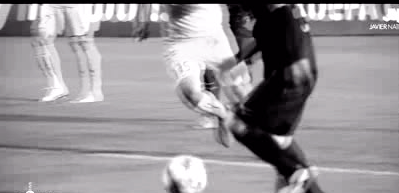
\includegraphics[scale=1]{imagenes/art1.png}

\subsection{Interpolación por Splines}

\begin{itemize}
\item Con seguridad, este hasta ahora es el método que genera los videos más fluidos.
\item Los movimientos de las cosas parecen naturales y no hay congelamientos ni transformaciones bruscas.
\item Esto se lo atribuimos a que el método en sí aprovecha todos los datos del pixel a tráves del tiempo para producir resultados mejores que tienen que ver con el marco teórico que le dan los polinomio interpoladores de Lagrange.
\item Eso si, siguen habiendo imágenes falsas a causa del movimiento y no son menores pero si ligeramente mejores que en la interpolación lineal.
\item Por ejemplo, en la instancia \textbf{skate}, los resultados son del estilo:
\end{itemize}

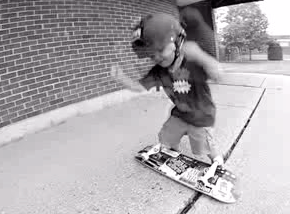
\includegraphics[scale=1]{imagenes/art2.png}

\subsection{Interpolación por Splines de a bloques de 4 pixeles}

\begin{itemize}
\item En este caso parece haber un retroceso de calidad con respecto al método anterior.
\item Los movimientos de las cosas parecen naturales.
\item Pero si hay congelamientos.
\item En particular, en el video \textbf{Messi} se nota claramente como la pelota se congela en algunos momentos.
\item Esto era de esperarse debido a los bloques de tamaño fijo ubicados a través del tiempo.
\end{itemize}


\newpage
\section{Conclusión}
%\setlength{\parindent}{15.0pt} % algún comando dejó en cero el parindent
En este trabajo pudimos no solo modelar el problema planteado, sino 
apreciar y aprovechar las propiedades del mismo para así resolverlo con los
métodos estudiados observando también las características de ellos.

Así mismo, cabe destacar que al realizar operaciones con aritmética finita,
tanto para la solución de los sistemas como para los valores evaluados en cada
interpolador, no podemos garantizar que los resultados obtenidos sean exactos,
pero dado que realizamos varias instancias de prueba con distintas metodologías,
pudimos ver que los valores que obtuvimos eran coherentes a su contexto.

Todos los métodos de interpolación realizados en este trabajo cumplieron con la
tarea de generar en mayor o menor medida el efecto de cámara lenta que
buscábamos cada uno con sus características particulares. Mediante la
experimentación pusimos bajo la lupa cada interpolador utilizado para así poder
compararlos entre sí.

Comenzamos nuestros experimentos probando el correcto funcionamiento de los
métodos implementados. Aquí además de ver mediante las cotas de precisión que
todos los métodos cumplían la tarea de interpolar las funciones predeterminadas
pudimos tener una primera visión sobre cómo se comportaba cada interpolador. El
más básico, por vecinos, efectivamente demostró tener la mayor cota de error
distanciándose ampliamente del resto, mientras que la interpolación lineal
obtuvo resultados similares a los obtenidos con splines. En este experimento en
particular, la interpolación mediante splines probó ser la de menor error,
superando a la lineal para funciones cuadráticas y cúbicas, donde a su vez se
pudo observar su relación con la interpolación por splines de a bloques, que con
bloques más grandes su cota se aproximaba a la del spline standard.

En la siguiente prueba, donde lo que se analizó fue el error producido al
elminar cuadros del video original e intentar recrearlos con nuestros
interpoladores, los resultados fueron similares al experimento anterior. Con
ambas fórmulas de cálculo de error (ECM y PSNR) se pudo ver cómo vecinos era el
método que peor se comportaba mientras que lineal y splines estuvieron
emparejados a lo largo de todas las instancias de prueba realizadas.

Finalmente, la búsqueda de artifacts en el video producido, de anomalías y
calidad final a nivel visual para el usuario resultó ser el punto determinante
para decidir cuál de los sistemas propuestos mejor se desempeña en la tarea de
proveer un efecto de cámara lenta. Los resultados acá dieron un giro completo
con respecto a las conclusiones que veníamos realizando respecto a las métricas
estudiadas. Para empezar, la interpolación de a vecinos dio mejores
resultados que la lineal en términos de cantidad de artifacts y calidad general
del video producido. El método por splines fue el que mejor llegó a producir la
sensación de cámara lenta, con algunas anomalías pero no lo suficientemente
signigicantes como las vistas en la interpolación lineal. Esto creemos que se
podría explicar con el hecho de que las métricas seleccionadas para decidir qué
interpolador era mejor estaban demasiado atadas a que interpolaran
correctamente sin contemplar cómo resultaba visualmente esta interpolación.

Por último, podemos mencionar como posibles desarrollos a futuro la búsqueda de
métricas que se centren más en el aspecto visual de los interpoladores,
distintas formas de interpolación o directamente métodos completamente
distintos, como lo sería considerar la aplicación de cuadrados mínimos, para
seguir comparando y buscando que se generen los menores artifacts posibles.


\newpage
%\bibliographystyle{plain}
\section{Referencias}
%\begingroup
%\renewcommand{\section}[2]{}
%\bibliography{informe}
%\endgroup

\newpage
\section{Enunciado}
%\documentclass[11pt, a4paper]{article}
\usepackage{a4wide,amsmath,amsfonts,graphicx,subcaption,tikz}
\usepackage[utf8]{inputenc} % para poder usar tildes en archivos UTF-8
\usepackage[spanish]{babel}
%\usepackage[ruled,vlined]{algorithm2e}

%\parindent = 0 pt
\parskip = 5 pt

\newcounter{row}
\newcounter{col}

\newcommand\setrow[3]{
	\setcounter{col}{1}
	\foreach \n in {#1, #2, #3} {
	\edef\x{\value{col} - 0.5}
	\edef\y{3.5 - \value{row}}
	\node[anchor=center] at (\x, \y) {\n};
	\stepcounter{col}
	}
	\stepcounter{row}
}

\newcommand\setrowaux[7]{
	\setcounter{col}{1}
	\foreach \n in {#1, #2, #3, #4, #5, #6, #7} {
	\edef\x{\value{col} - 0.5}
	\edef\y{7.5 - \value{row}}
	\node[anchor=center] at (\x, \y) {\n};
	\stepcounter{col}
	}
	\stepcounter{row}
}

\newcommand{\real}{\mathbb{R}}

\begin{document}
\begin{center}
\begin{tabular}{r|cr}
 \begin{tabular}{c}
{\large\bf\textsf{\ M\'etodos Num\'ericos\ }}\\ 
Segundo Cuatrimestre 2015\\
{\bf Trabajo Pr\'actico 3}\\
\end{tabular} &
\begin{tabular}{@{} p{1.6cm} @{}}
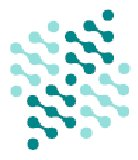
\includegraphics[width=1.6cm]{logodpt.jpg}
\end{tabular} &
\begin{tabular}{l @{}}
 \emph{Departamento de Computaci\'on} \\
 \emph{Facultad de Ciencias Exactas y Naturales} \\
 \emph{Universidad de Buenos Aires} \\
\end{tabular} 
\end{tabular}
\vskip 10pt
\textbf{\Large \emph{Un juego de niños}}\\
\vspace{0.5cm}
\end{center}

\vskip 10pt
\hrule
\vskip 5pt

{\bf\noindent Introducci\'on}

¿Quién nunca ha visto un video gracioso de bebés? El éxito de esas producciones audiovisuales ha sido tal que el sitio youborn.com es uno de los más visitados diariamente. Los dueños de este gran sitio, encargado de la importantísima tarea de llevar videos graciosos con bebés a todo el mundo, nos ha pedido que mejoremos su sistema de reproducción de videos.

Su objetivo es tener videos en cámara lenta (ya que todos deseamos tener lujo de detalle en las expresiones de los chiquilines en esos videos) pero teniendo en cuenta que las conexiones a internet no necesariamente son capaces de transportar la gran cantidad de datos que implica un video en \textit{slow motion}. La gran idea es minimizar la dependencia de la velocidad de conexi\'on y s\'olo enviar el video original. Una vez que el usuario recibe esos datos, todo el trabajo de la cámara lenta puede hacerse de modo offline del lado del cliente, optimizando los tiempos de transferencia. Para tal fin utilizaremos técnicas de interpolación, buscando generar, entre cada par de cuadros del video original, otros ficticios que nos ayuden a generar un efecto de slow motion.


\vskip 5pt

{\bf\noindent Definici\'on del problema y metodolog\'ia}

Para resolver el problema planteado en la secci\'on anterior, se considera el siguiente contexto. Un video está compuesto por cuadros (denominados también \textit{frames} en inglés) donde cada uno de ellos es una imagen. Al reproducirse rápidamente una después de la otra percibimos el efecto de movimiento a partir de tener un ``buen frame rate'', es decir una alta cantidad de cuadros por segundo o fps (frames per second). Por lo general las tomas de cámara lenta se generan con cámaras que permiten tomar altísimos números de cuadros por segundo, unos 100 o m\'as en comparaci\'on con entre 24 y 30 que se utilizan normalmente. 

En el caso del trabajo práctico crearemos una cámara lenta sobre un video grabado normalmente. Para ello colocaremos más cuadros entre cada par de cuadros consecutivos del video original de forma que representen la información que debería haber en la transición y reproduciremos el resultado a la misma velocidad que el original. Las im\'agenes correspondientes a cada cuadro est\'an conformadas por p\'ixeles. En particular, en este trabajo utilizaremos im\'agenes en escala de grises para disminuir los costos en tiempo necesarios para procesar los datos y simplificar la implementaci\'on; sin embargo, la misma idea puede ser utilizada para videos en color. 

El objetivo del trabajo es generar, para cada posici\'on $(i,j)$, los valores de los cuadros agregados en funci\'on de los cuadros conocidos. Lo que haremos ser\'a interpolar en el tiempo y para ello, se propone considerar al menos los siguientes tres m\'etodos de interpolaci\'on:

\begin{enumerate}
\item \emph{Vecino m\'as cercano:} Consiste en rellenar el nuevo cuadro replicando los valores de los p\'ixeles del cuadro original que se encuentra más cerca. \label{item:nn}
\item \emph{Interpolaci\'on lineal:} Consiste en rellenar los p\'ixeles utilizando interpolaciones lineales entre p\'ixeles de cuadros originales consecutivos. \label{item:lineal}
\item \emph{Interpolaci\'on por Splines:} Simliar al anterior, pero considerando interpolar utilizando splines y tomando una cantidad de cuadros mayor. Una alternativa a considerar es tomar la informaci\'on de bloques de un tama\~no fijo (por ejemplo, 4 cuadros, 8 cuadros, etc.), con el tama\~no de bloque a ser determinado experimentalmente. \label{item:spline}
\end{enumerate}


Cada m\'etodo tiene sus propias caracter\'isticas, ventajas y desventajas particulares. Para realizar un an\'alisis cuantitativo, llamamos $F$ al frame del video real (ideal) que deber\'iamos obtener con nuestro algoritmo, y sea $\bar{F}$ al frame del video efectivamente construido. Consideramos entonces dos medidas, directamente relacionadas entre ellas, como el \emph{Error Cuadr\'atico Medio} (ECM) y \emph{Peak to Signal Noise Ratio} (PSNR), denotados por $\texttt{ECM}(F,\bar{F})$ y $\texttt{PSNR}(F,\bar{F})$, respectivamente, y definidos como:
\begin{equation}
\texttt{ECM}(F,\bar{F}) = \frac{1}{mn}\sum_{i=1}^m\sum_{j = 1}^n |F_{k_{ij}} - \bar{F}_{k_{ij}}|^2 \label{eq:ecm}
\end{equation}
\noindent y
\begin{equation}
\texttt{PSNR}(F,\bar{F}) = 10 \log_{10}\bigg(\frac{255^2}{\texttt{ECM}(F,\bar{F})}\bigg). \label{eq:psnr}
\end{equation}

Donde $m$ es la cantidad de filas de p\'ixeles en cada imagen y $n$ es la cantidad de columnas. Esta métrica puede extenderse para todo el video.

En conjunto con los valores obtenidos para estas m\'etricas, es importante además realizar un an\'alisis del tiempo de ejecuci\'on de cada m\'etodo y los denominados \emph{artifacts} que produce cada uno de ellos. Se denominan \emph{artifacts} a aquellos errores visuales resultantes de la aplicaci\'on de un m\'etodo o t\'ecnica. La b\'usqueda de este tipo de errores complementa el estudio cuantitativo mencionado anteriormente incorporando un an\'alisis cualitativo (y eventualmente subjetivo) sobre las im\'agenes generadas.

\vskip 5pt

{\bf\noindent Enunciado}

Se pide implementar un programa en \verb-C- o \verb-C++- que implemente como m\'inimo los tres m\'etodos mencionados anteriormente y que dado un video y una cantidad de cuadros a agregar aplique estas t\'ecnicas para generar un video de cámara lenta. A su vez, es necesario explicar en detalle c\'omo se utilizan y aplican los m\'etodos descriptos en \ref{item:nn}, \ref{item:lineal} y \ref{item:spline} (y todos aquellos otros m\'etodos que decidan considerar opcionalmente) en el contexto propuesto. Los grupos deben a su vez plantear, describir y realizar de forma adecuada los experimentos que consideren pertinentes para la evaluaci\'on de los m\'etodos, justificando debidamente las decisiones tomadas y analizando en detalle los resultados obtenidos as\'i como tambi\'en plantear qu\'e pruebas realizaron para convencerse de que los m\'etodos funcionan correctamente.


{\bf\noindent Programa y formato de entrada}

Se deberán entregar los archivos fuentes que contengan la resolución del trabajo práctico. El ejecutable tomará cuatro parámetros por línea de comando que serán el archivo de entrada, el archivo de salida, el método a ejecutar (0 para vecinos más cercanos, 1 para lineal, 2 para splines y otros números si consideran más métodos) y la cantidad de cuadros a agregar entre cada par del video original.

Tanto el archivo de entrada como el de salida tendrán la siguiente estructura:

\begin{itemize}
  \item En la primera línea está la cantidad de cuadros que tiene el video (\verb|c|).
  \item En la segunda línea está el tamaño del cuadro donde el primer número es la cantidad de filas y el segundo es la cantidad de columnas (\verb|height width|).
  \item En la tercera línea está el framerate del video (\verb|f|).
  \item A partir de allí siguen las imágenes del video una después de la otra en forma de matriz. Las primeras \verb|height| l\'ineas son las filas de la primera imagen donde cada una tiene \verb|width| n\'umeros correspondientes a los valores de cada píxel en esa fila. Luego siguen las filas de la siguiente imagen y as\'i sucesivamente.
\end{itemize}

Además se presentan herramientas en Matlab para transformar videos (la herramienta fue probada con la extensión .avi pero es posible que funcione para otras) en archivos de entrada para el enunciado y archivos de salida en videos para poder observar el resultado visualmente. También se recomienda leer el archivo de README sobre la utilización.


\vskip 0.5 cm
\hrule
\vskip 0.2 cm

{\bf Sobre la entrega}
\begin{itemize}
\item \textsc{Formato electr\'onico:} Martes 10 de Noviembre de 2015, {\bf{\underline{hasta las 23:59}}}, enviando el trabajo
(\texttt{informe} + \texttt{c\'odigo}) a \texttt{metnum.lab@gmail.com}. El \texttt{asunto} del email debe comenzar con el texto \verb|[TP3]| seguido
de la lista de apellidos de los integrantes del grupo. Ejemplo: \texttt{[TP3] Artuso, Belloli, Landini}
\item \textsc{Formato f\'isico:} Mi\'ercoles 11 de Noviembre de 2015, en la clase pr\'actica.
\end{itemize}


\end{document}

\newpage
\appendix
%%\newpage
\section{Código C++} \label{sec:codigo}

\newcommand{\codelst}{\begingroup
  \catcode`_=12 \docodelst}
\newcommand{\docodelst}[1]{%
  \lstinputlisting[language=C++]{#1}%
  \endgroup
}

\subsection*{video.cpp}
\codelst{../src/video.cpp}
\subsection*{interpolador.h}
\codelst{../src/interpolador.h}
\subsection*{spline.cpp}
\codelst{../src/spline.cpp}
\subsection*{lineal.h}
\codelst{../src/lineal.cpp}
\subsection*{vecinos.cpp}
\codelst{../src/vecinos.cpp}
\subsection*{multi_spline.cpp}
\codelst{../src/multi_spline.cpp}
\subsection*{test_utils.h}
\codelst{../src/test_utils.h}


\end{document}
